\documentclass[a4paper,12pt]{article} % добавить leqno в [] для нумерации слева
\usepackage[a4paper,top=1.3cm,bottom=2cm,left=1.5cm,right=1.5cm,marginparwidth=0.75cm]{geometry}
%%% Работа с русским языком
\usepackage{cmap}					% поиск в PDF
\usepackage{mathtext} 				% русские буквы в фомулах
\usepackage[T2A]{fontenc}			% кодировка
\usepackage[utf8]{inputenc}			% кодировка исходного текста
\usepackage[english,russian]{babel}	% локализация и переносы
\usepackage{multirow}

\usepackage{graphicx}

\usepackage{wrapfig}
\usepackage{tabularx}

\usepackage{hyperref}
\usepackage[rgb]{xcolor}
\hypersetup{
colorlinks=true,urlcolor=blue
}

%%% Дополнительная работа с математикой
\usepackage{amsmath,amsfonts,amssymb,amsthm,mathtools} % AMS
\usepackage{icomma} % "Умная" запятая: $0,2$ --- число, $0, 2$ --- перечисление

%% Номера формул
\mathtoolsset{showonlyrefs=true} % Показывать номера только у тех формул, на которые есть \eqref{} в тексте.

%% Шрифты
\usepackage{euscript}	 % Шрифт Евклид
\usepackage{mathrsfs} % Красивый матшрифт

%% Свои команды
\DeclareMathOperator{\sgn}{\mathop{sgn}}

%% Перенос знаков в формулах (по Львовскому)
\newcommand*{\hm}[1]{#1\nobreak\discretionary{}
{\hbox{$\mathsurround=0pt #1$}}{}}

%% Графики
\usepackage{tikz}
\usepackage{pgfplots}
\pgfplotsset{compat=1.9}

\date{\today}

\begin{document}

\begin{titlepage}
	\begin{center}
		{\large МОСКОВСКИЙ ФИЗИКО-ТЕХНИЧЕСКИЙ ИНСТИТУТ (НАЦИОНАЛЬНЫЙ ИССЛЕДОВАТЕЛЬСКИЙ УНИВЕРСИТЕТ)}
	\end{center}
	\begin{center}
		{\large Физтех-школа аэрокосмических технологий}
	\end{center}
	
	
	\vspace{4.5cm}
	{\huge
		\begin{center}
			{\bf Отчёт о выполнении лабораторной работы 2.2.6}\\
			Определение энергии активации по температурной зависимости вязкости жидкости
		\end{center}
	}
	\vspace{1cm}
	\begin{center}
		{\large Соболевский Федор Александрович \\
			\vspace{0.2cm}
			Б03-109}
	\end{center}
	\vspace{8cm}
	\begin{center}
		Февраль 2022
	\end{center}
\end{titlepage}

\section{Аннотация}

В данной работе рассмотрен метод определения энергии активации молекул жидкости по зависимости вязкости жидкости от её температуры. Измерены скорости падения шариков малых радиусов в жидкости при разных значениях температуры. Для вычисления вязкости применена формула Стокса. Вычислены и проанализированы погрешности измерений и характерные величины, описывающие процесс падения, для обоснования применимости используемых в работе соотношений.

\section{Теоретические сведения}

\subsection{Энергия активации}

По своим свойствам жидкости похожи и на твёрдые тела, и на газы. Как и в твёрдых телах, каждая молекула жидкости находится в потенциальной яме электрического поля, создаваемого другими молекулами. Подобно молекулам газа, в жидкости молекулы могут смещаться относительно других. Для преодоления участков с большей потенциальной энергией, чем средняя кинетическая энергия молекул, частица должна вследствие флуктуаций приобрести дополнительную энергию. Величина этой дополнительной энергии называется энергией активации и обозначается $W$. Вследствие необходимости дополнительной энергии перемещения молекул жидкости относительно друг друга происходят сравнительно редко и тем реже, чем больше величина $W$.

Описанный характер движения молекул в жидкостях объясняет их большую, чем у газов, вязкость. В газах вязкость объясняется происходящим при тепловом движении молекул переносом количества направленного движения. В жидкостях такие переходы существенно замедлены. Согласно формуле Больцмана, количество молекул, имеющих энергии больше $W$, зависит экспоненциально от $W$. Температурная зависимость вязкости от энергии активации определяется как

\begin{equation}
    \eta = Ae^{\frac{W}{kT}},
    \label{viscocity}
\end{equation}

где $A$ - некоторый коэффициент. При приближениях, использованных при выводе формулы \eqref{viscocity}, $A$ можно считать постоянным, поэтому величину $W$ можно найти из коэффициента наклона прямой в зависимости $\ln{\eta}$ от $\frac{1}{T}$:

\begin{equation}
    W = k\frac{d(\ln{\eta})}{d(\frac{1}{T})}.
    \label{activationEnergy}
\end{equation}

Также по отклонению полученных результатов от аппроксимирующей прямой можно оценить погрешность измерений и применимость используемых приближений.

\subsection{Метод Стокса}

Для определения вязкости жидкости в работе используется метод Стокса, основанный на измерении скорости падения шарика в жидкости. На всякое тело, движущееся в вязкой среде, действует сила сопротивления, зависящая от многих параметров: вязкости жидкости, формы тела, характера обтекания и т.д. Стоксом было получено строгое решение задачи движения шарика при его ламинарном обтекании безграничной жидкостью: в этом случае сила сопротивления определяется формулой

\begin{equation}
    F = 6\pi\eta r v,
    \label{Stokes}
\end{equation}

где $\eta$ - вязкость жидкости, $r$ - радиус шарика, $v$ - его скорость. Данная формула работает при достаточно малых значениях $v$ и $r$. Оценка достаточности малости данных величин не может быть получена теоретически и должна быть произведена в ходе эксперимента.

При падении в жидкости на шарик действуют три силы: сила тяжести, сила Архимеда и сила вязкости. По второму закону Ньютона:

\begin{equation}
    Vg(\rho - \rho_\text{ж}) - 6\pi\eta rv = V\rho\frac{dv}{dt},
    \label{movementEq}
\end{equation}

где $V$ - объём шарика, $\rho$ - его плотность, $\rho_\text{ж}$ - плотность жидкости. Плотность жидкости (в данном опыте - глицерина) при данной температуре можно найти по графику на рис. \ref{fig:graph}.

\begin{figure}
    \centering
    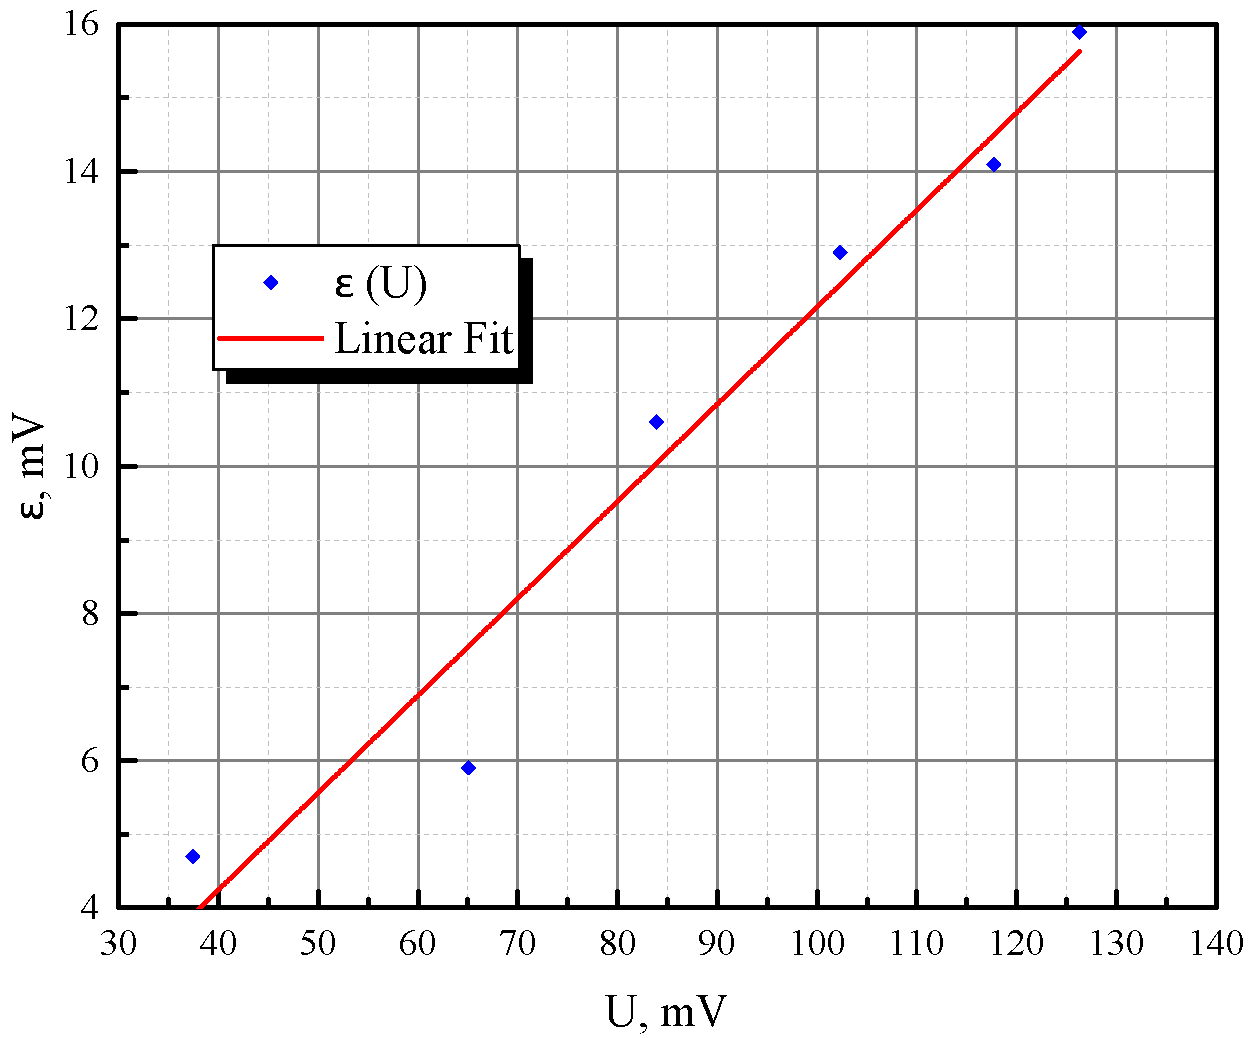
\includegraphics[width = 0.55\textwidth]{graph.PNG}
    \caption{Зависимость плотности глицерина от температуры}
    \label{fig:graph}
\end{figure}

Решая уравнение \eqref{movementEq}, находим

\begin{equation}
    v(t) = v_\text{уст} - (v_\text{уст} - v_0)e^{-\frac{t}{\tau}}.
    \label{velocity}
\end{equation}

В формуле \eqref{velocity} $v_0$ - скорость шарика в начальный момент времени,

\begin{equation}
    v_\text{уст} = \frac{Vg(\rho - \rho_\text{ж})}{6\pi\eta r} = \frac{2}{9}gr^2\frac{\rho - \rho_\text{ж}}{\eta}
    \label{stableVelocity}
\end{equation}

- установившаяся скорость,

\begin{equation}
    \tau = \frac{V\rho}{6\pi\eta r} = \frac{2}{9} \frac{r^2\rho}{\eta}
\end{equation}

- время релаксации. Если время релаксации значительно меньше времени падения, то процесс установления скорости можно считать законченным. Измеряя на опыте установившуюся скорость падения шариков, можно определить вязкость жидкости по формуле, следующей из формулы \eqref{stableVelocity}:

\begin{equation}
    \eta = \frac{2}{9}gr^2\frac{\rho - \rho_\text{ж}}{v_\text{уст}}.
    \label{finalViscocity}
\end{equation}

При необходимости учесть влияние стенок сосуда на движение шариков следует использовать более точную формулу.

\begin{equation}
    \eta = \frac{2}{9}gr^2\frac{\rho - \rho_\text{ж}}{(1 + 2,4\frac{r}{R})v_\text{уст}},
\end{equation}

где $R$ - радиус сосуда. Для небольших шариков отличие данной формулы от \eqref{finalViscocity} незначительно и не приниматься во внимание.

Применимость формулы Стокса можно также исследовать теоретически. Характер обтекания шарика жидкостью определяется значением числа Рейнольдса $\text{Re} = \frac{vr\rho_\text{ж}}{\eta}$. Обтекание можно считать ламинарным при достаточно малых значениях Re (меньших 0,5). Также для оценки применимости метода Стокса полезно вычислить время релаксации $\tau$ и пройденный путь $S$, который можно вычислить интегрированием \eqref{velocity} (можно принять $v_0 = 0$ для простоты, т.к. это с хорошей точностью выполняется в опытах):

\begin{equation}
    S = v_\text{уст}\tau(\frac{t}{\tau} - 1 + e^{-\frac{t}{\tau}}).
\end{equation}

Отсюда видно, что $S \gg v_\text{уст}\tau$ при $t \gg \tau$. Последнее неравенство определяет допустимое расстояние между границей жидкости и верхней меткой.

\subsection{Экспериментальная установка}

\begin{figure}
    \centering
    \includegraphics[width = 0.55\textwidth]{setup.PNG}
    \caption{Схема установки для определения коэффициента вязкости жидкости}
    \label{fig:setup}
\end{figure}

\begin{figure}
    \centering
    \includegraphics[width = 0.4\textwidth]{photo.PNG}
    \caption{Термостат}
    \label{fig:photo}
\end{figure}

Для измерений используется стеклянный цилиндрический сосуд, заполненный глицерином (исследуемой жидкостью) и помещённый в рубашку, омываемую водой из термостата для поддержания постоянной заданной температуры жидкости. Схема экспериментальной установки показана на рис. \ref{fig:setup}. Внешний вид термостата показан на рис. \ref{fig:photo}. Обозначения: 1 - блок терморегулирования; 2 - ванна; 3 - индикаторное табло; 5 - кнопка переключения режимов установки/контроля температуры; 6 - индикатор уровня жидкости; 7 - индикатор включения нагревателя; 8 - сетевой выключатель прибора; 9 - крышка; 10 - входной и выходной патрубки насоса; 11 - входной и выходной патрубки теплообменника. 

Ванна представляет собой емкость из нержавеющей стали, установленную в наружный кожух. В блоке терморегулирования расположены: насос для обеспечения перемешивания рабочей жидкости и перекачки её во внешний контур, нагреватель, датчик температуры, датчик уровня жидкости, элементы управления и индикации, необходимые для надёжной работы.

\section{Оборудование и экспериментальные погрешности}

\textbf{В работе использовались:} стеклянный цилиндр с исследуемой жидкостью (глицерин); термостат; секундомер; микроскоп; мелкие стеклянные и стальные шарики (диаметром около 1 мм).

\textbf{Инструментальные погрешности:}

\begin{itemize}
    \item \textbf{Секундомер:} $\Delta_\text{с} = 0,01 $ c;
    \item \textbf{Микроскоп:} $\Delta_\text{м} = 0,05 $ мм.
\end{itemize}

\section{Результаты измерений и обработка экспериментальных данных}

\subsection{Измерение скорости падения шариков и вычисление вязкости}

В данной работе измерялось время прохождения шариками двух участков в жидкости длиной $l = 10$ см каждый. Затем полученное значение скорости на каждом из участков усреднялось для получения более точного результата.

\begin{table}[]
    \centering
    \begin{tabular}{|c|c|c|c|c|c|c|c|c|c|c|} \hline
        \multicolumn{11}{|c|}{Сталь: $\rho_1 = 7,8$ г/$\text{см}^3$}\\ \hline
        № шарика & 1 & 2 & 3 & 4 & 5 & 6 & 7 & 8 & 9 & 10 \\ \hline
        $d$, мм & 0,55 & 0,55 & 0,5 & 0,75 & 0,65 & 0,85 & 0,85 & 0,65 & 0,65 & 0,65 \\ \hline
        $ r $, мм & 0,275 & 0,275 & 0,25 & 0,375 & 0,325 & 0,425 & 0,425 & 0,325 & 0,325 & 0,325 \\ \hline
        \multicolumn{11}{|c|}{Стекло: $\rho_2 = 2,5$ г/$\text{см}^3$}\\ \hline
        № шарика & 1 & 2 & 3 & 4 & 5 & 6 & 7 & 8 & 9 & 10 \\ \hline
        $d$, мм & 2,1 & 2,1 & 2,05 & 2,1 & 2,1 & 2,1 & 2,1 & 2,1 & 2,1 & 2,15 \\ \hline
        $ r $, мм & 1,05 & 1,05 & 1,025 & 1,05 & 1,05 & 1,05 & 1,05 & 1,05 & 1,05 & 1,075 \\ \hline
    \end{tabular}
    \caption{Размеры и плотности шариков}
    \label{tab:dimensions}
\end{table}

Размеры использованных в работе шариков и плотности их материалов указаны в таблице \ref{tab:dimensions}. Далее были измерены скорости падения шариков в глицерине при разных температурах и найдены по формуле \eqref{finalViscocity} соответствующие значения вязкости. Оценены также число Рейнольдса, время и путь релаксации для каждого опыта. Полученные результаты представлены в таблице \ref{tab:results}. 

\begin{table}[]
    \centering
    \begin{tabular}{|c|c|c|c|c|c|c|c|} \hline
        \multicolumn{8}{|c|}{$T_1 = 294,75 $ К, $\rho_\text{ж} = 1,259$ г/$\text{см}^3$} \\ \hline
        № шарика & $t_1$, с & $t_2$, с & $v_\text{уст}$, мм/с & $\eta$, Па$\cdot$с & Re$\cdot 10^3$ & $\tau$, $10^{-3}$ с & $S$, $10^{-3}$ мм  \\ \hline
        1 & 79,15 & 80,29 & 1,25 & 0,860 & 0,5 & 0,2 & 0,2 \\ \hline
        2 & 76,65 & 78,03 & 1,29 & 0,834 & 0,5 & 0,2 & 0,2 \\ \hline
        11 & 33,34 & 33,21 & 3,01 & 0,992 & 4,0 & 0,6 & 1,9 \\ \hline
        12 & 32,64 & 32,57 & 3,07 & 0,973 & 4,2 & 0,6 & 1,9 \\ \hline
        \multicolumn{8}{|c|}{$\overline{\eta}_1 = 0,915$ Па$\cdot$с} \\ \hline
        \multicolumn{8}{|c|}{$T_2 = 300$ К, $\rho_\text{ж} = 1,257$ г/$\text{см}^3$} \\ \hline
        № шарика & $t_1$, с & $t_2$, с & $v_\text{уст}$, мм/с & $\eta$, Па$\cdot$с & Re$\cdot 10^3$ & $\tau$, $10^{-3}$ с & $S$, $10^{-3}$ мм  \\ \hline
        3 & 73,48 & 72,68 & 1,37 & 0,651 & 0,7 & 0,2 & 0,2 \\ \hline
        4 & 27,36 & 27,15 & 3,67 & 0,547 & 3,2 & 0,4 & 1,6 \\ \hline
        13 & 22,38 & 22,10 & 4,50 & 0,633 & 9,1 & 0,9 & 4,1 \\ \hline
        14 & 21,67 & 22.04 & 4,58 & 0,653 & 9,2 & 0,9 & 4,3 \\ \hline
        \multicolumn{8}{|c|}{$\overline{\eta}_2 = 0,621$ Па$\cdot$с} \\ \hline
        \multicolumn{8}{|c|}{$T_3 = 305$ К, $\rho_\text{ж} = 1,255$ г/$\text{см}^3$} \\ \hline
        № шарика & $t_1$, с & $t_2$, с & $v_\text{уст}$, мм/с & $\eta$, Па$\cdot$с & Re$\cdot 10^3$ & $\tau$, $10^{-3}$ с & $S$, $10^{-3}$ мм  \\ \hline
        5 & 28,74 & 28,20 & 3,51 & 0,429 & 3,3 & 0,4 & 1,5 \\ \hline
        6 & 17,41 & 17,79 & 5,68 & 0,454 & 6,7 & 0,7 & 3,9 \\ \hline
        15 & 15,01 & 15,21 & 6,62 & 0,452 & 19,3 & 1,4 & 9,0 \\ \hline
        16 & 17,30 & 14,13 & 6,36 & 0,470 & 17,8 & 1,3 & 8,3 \\ \hline
        \multicolumn{8}{|c|}{$\overline{\eta}_3 = 0,451$ Па$\cdot$с} \\ \hline
        \multicolumn{8}{|c|}{$T_4 = 310$ К, $\rho_\text{ж} = 1,253$ г/$\text{см}^3$} \\ \hline
        № шарика & $t_1$, с & $t_2$, с & $v_\text{уст}$, мм/с & $\eta$, Па$\cdot$с & Re$\cdot 10^3$ & $\tau$, $10^{-3}$ с & $S$, $10^{-3}$ мм  \\ \hline
        7 & 13,28 & 11,69 & 8,01 & 0,322 & 13,3 & 1,0 & 7,8 \\ \hline
        8 & 21,39 & 21,69 & 4,64 & 0,325 & 5,8 & 0,6 & 2,6 \\ \hline
        17 & 10,25 & 11,05 & 9,39 & 0,319 & 38,7 & 1,9 & 18,0 \\ \hline
        18 & 10,16 & 10,45 & 9,70 & 0,309 & 41,3 & 2,0 & 19,2 \\ \hline
        \multicolumn{8}{|c|}{$\overline{\eta}_4 = 0,319$ Па$\cdot$с} \\ \hline
        \multicolumn{8}{|c|}{$T_5 = 315$ К, $\rho_\text{ж} = 1,250$ г/$\text{см}^3$} \\ \hline
        № шарика & $t_1$, с & $t_2$, с & $v_\text{уст}$, мм/с & $\eta$, Па$\cdot$с & Re$\cdot 10^3$ & $\tau$, $10^{-3}$ с & $S$, $10^{-3}$ мм  \\ \hline
        9 & 14,53 & 15,30 & 6,70 & 0,225 & 12,1 & 0,8 & 5,5 \\ \hline
        10 & 14,40 & 14,12 & 14,26 & 0,215 & 13,2 & 0,9 & 6,0 \\ \hline
        19 & 7,29 & 7,20 & 13,80 & 0,218 & 83,2 & 2,8 & 38,8 \\ \hline
        20 & 7,23 & 7,22 & 13,84 & 0,228 & 81,7 & 2,8 & 39,1 \\ \hline
        \multicolumn{8}{|c|}{$\overline{\eta}_5 = 0,221$ Па$\cdot$с} \\ \hline
    \end{tabular}
    \caption{Результаты измерения установившихся скоростей, вязкости и характерных величин при падении шариков в глицерине}
    \label{tab:results}
\end{table}

Как видно из результатов измерений, время и путь релаксации значительно меньше времени движения и пройденного шариком пути соответственно в каждом опыте. Число Рейнольдса во всех случаях оказалось на порядок меньше границы ламинарности течения. Это говорит о применимости использованных при измерениях соотношений.

\subsection{Вычисление энергии активации}

Зависимость $\ln{\eta}$ от $1/T$ представлена в таблице \ref{tab:graphData} и на рисунке \ref{graph}. Как видно на графике, полученные значения хорошо ложатся на аппроксимирующую прямую. Коэффициент наклона аппроксимирующей прямой, то есть $d(\ln \eta)/d(1/T)$, и погрешность его определения можно вычислить, воспользовавшись методом наименьших квадратов:

\begin{table}[]
    \centering
    \begin{tabular}{|c|c|c|c|c|c|} \hline
        $1/T$, $10^{-3}$ $\text{К}^{-1}$ & 3,39 & 3,33 & 3,28 & 3,23 & 3,18 \\ \hline
        $\ln{\eta}$ & -0,089 & -0,476 & -0,796 & -1,143 & -1,510 \\ \hline
    \end{tabular}
    \caption{Зависимость вязкости от температуры}
    \label{tab:graphData}
\end{table}

\begin{equation}
    \frac{d(\ln \eta)}{d(1/T)} = \frac{\langle \ln{\eta}\cdot 1/T\rangle-\langle \ln{\eta}\rangle \langle 1/T\rangle}{\langle (1/T)^2\rangle - \langle 1/T\rangle^2} = 6,447 \cdot 10^3 \text{ К},
\end{equation}

\begin{equation}
    \sigma = \sqrt{\frac{1}{5}\left(\frac{\langle (\ln{\eta})^2 \rangle - \langle \ln{\eta} \rangle^2}{\langle (1/T)^2 \rangle - \langle 1/T \rangle^2} - (\frac{d(\ln \eta)}{d(1/T)})^2 \right) } = 0,094 \cdot 10^3 \text{ К}.
\end{equation}

\begin{figure}
\centering
\resizebox {0.7\textwidth} {!} {
\begin{tikzpicture}
\begin{axis}[ xlabel = {$1/T$, $10^{-3}$ $\text{К}^{-1}$}, ylabel = {$\ln{\eta}$}, xmin = 3.15, xmax = 3.45, ymin = -1.65, ymax = 0]
\addplot[color=black, mark=x, only marks] coordinates{(3.39, -0.089)(3.33, -0.476)(3.28, -0.796)(3.23, -1.143)(3.18, -1.51)};
\addplot[color=blue] coordinates{(3.18, -1.5)(3.39, -0.08)};
\end{axis}
\end{tikzpicture}
}
\caption{Зависимость вязкости от температуры}
\label{graph}
\end{figure}

Отсюда энергия активации по формуле \eqref{activationEnergy}

\begin{equation}
    W = k\frac{d(\ln{\eta})}{d(\frac{1}{T})} = 8,897 \cdot 10^{-20} \text{ Дж}.
\end{equation}

\section{Обсуждение результатов и выводы}

В ходе вычислений было установлено, что рассмотренные соотношения выполняются с достаточной точностью в экспериментах. Отклонение зависимости $\ln{\eta}$ от $1/T$ от линейной оказалось пренебрежимо мало. Это говорит о том, что приближения, при которых была выведена формула \eqref{viscocity}, верны для малых температурных диапазонов ($\pm 30$ К). 

Отклонение значения энергии активации молекул глицерина от табличного (($8,341 \pm 0,087)\cdot 10^{-20}$ Дж) составило около 6\%. Данное отклонение может указывать на некоторое отличие исследуемой жидкости от чистого глицерина либо на ошибку измерений, однако оно достаточно мало, чтобы подтвердить применимость рассмотренных соотношений для измерения энергии активации молекул жидкости.

\end{document}
